\clearpage
\SourceLeaf{262}%
\begin{center}
\textbf{[DIE SPH\"ARISCHE UND DIE NICHT-EUKLIDISCHE GEOMETRIE.]}

\smallskip

\end{center}

\[
\tag*{I.} ga\,.\,\partial b - \sin B\,.\,\partial c + fc\,.\,\cos B\,.\,\partial A = 0
\]

\[
\tag*{II.} gb\,.\,\partial a - \sin A\,.\,\partial c + fc\,.\,\cos A\,.\,\partial B = 0
\]

\noindent durch Construction;

\[
\tag*{III.} \sin B\,.\,\partial a - ga\,.\,\cos B\,.\,\partial b - fc\,.\,\partial A = 0
\]

\[
\tag*{IV.} gb\,.\,\cos A\,.\,\partial a - \sin A\,.\,\partial b + fc\,.\,\partial B = 0
\]

\noindent gleichfalls durch Construction.

\begin{center}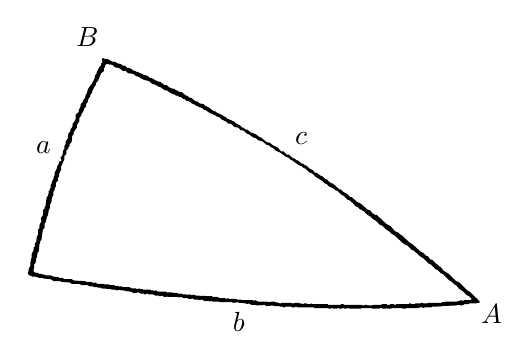
\begin{tikzpicture}[x=0.00833333cm,y=-0.00833333cm]
\fill[even odd rule] (41,408) -- (43,412) -- (47,413) -- (48,414) -- (53,414) -- (54,415) -- (57,415) -- (58,416) -- (64,416) -- (65,417) -- (76,418) -- (81,421) -- (91,421) -- (92,422) -- (105,423) -- (108,425) -- (120,425) -- (123,427) -- (133,427) -- (135,429) -- (141,429) -- (142,430) -- (147,430) -- (148,431) -- (152,431) -- (153,432) -- (168,433) -- (169,434) -- (175,434) -- (176,435) -- (182,434) -- (183,435) -- (188,435) -- (189,436) -- (199,437) -- (202,439) -- (207,439) -- (208,438) -- (210,438) -- (213,440) -- (218,440) -- (219,441) -- (221,441) -- (222,440) -- (224,440) -- (225,441) -- (232,441) -- (236,443) -- (241,443) -- (242,444) -- (246,443) -- (249,445) -- (252,445) -- (253,444) -- (255,445) -- (271,445) -- (272,446) -- (275,445) -- (279,447) -- (285,447) -- (286,448) -- (290,448) -- (292,447) -- (295,449) -- (301,449) -- (302,450) -- (307,449) -- (310,451) -- (317,451) -- (318,452) -- (322,451) -- (323,452) -- (333,452) -- (334,453) -- (353,453) -- (354,454) -- (362,453) -- (363,454) -- (370,454) -- (371,455) -- (374,455) -- (375,456) -- (378,455) -- (382,457) -- (389,457) -- (390,458) -- (393,458) -- (394,457) -- (396,458) -- (402,457) -- (405,459) -- (416,458) -- (417,459) -- (425,459) -- (426,460) -- (430,460) -- (431,461) -- (433,461) -- (434,460) -- (443,460) -- (444,461) -- (448,461) -- (449,460) -- (451,460) -- (452,461) -- (477,461) -- (478,462) -- (499,462) -- (500,463) -- (503,463) -- (504,462) -- (506,462) -- (507,463) -- (512,463) -- (513,462) -- (515,462) -- (516,463) -- (520,463) -- (521,462) -- (523,462) -- (524,463) -- (527,463) -- (528,462) -- (530,462) -- (531,463) -- (549,463) -- (550,462) -- (565,462) -- (566,463) -- (577,463) -- (578,462) -- (581,462) -- (582,463) -- (587,463) -- (588,462) -- (590,463) -- (595,463) -- (596,462) -- (612,462) -- (613,463) -- (617,463) -- (618,462) -- (637,462) -- (638,461) -- (643,461) -- (645,462) -- (646,461) -- (649,461) -- (650,460) -- (651,461) -- (656,461) -- (657,460) -- (666,460) -- (667,459) -- (670,460) -- (671,459) -- (695,458) -- (696,457) -- (700,457) -- (701,458) -- (703,458) -- (707,456) -- (713,456) -- (714,455) -- (725,455) -- (726,454) -- (729,454) -- (730,453) -- (730,452) -- (726,448) -- (726,447) -- (725,447) -- (716,438) -- (711,435) -- (699,423) -- (694,421) -- (683,410) -- (675,405) -- (670,399) -- (669,399) -- (665,395) -- (664,395) -- (657,388) -- (655,388) -- (651,383) -- (649,383) -- (644,378) -- (640,376) -- (628,365) -- (623,362) -- (610,350) -- (609,350) -- (606,347) -- (601,345) -- (594,337) -- (588,334) -- (573,320) -- (570,320) -- (568,318) -- (567,318) -- (563,313) -- (559,312) -- (549,303) -- (543,300) -- (535,293) -- (533,293) -- (528,288) -- (522,285) -- (518,281) -- (516,281) -- (506,272) -- (504,272) -- (502,270) -- (501,270) -- (497,266) -- (494,265) -- (490,261) -- (487,260) -- (482,256) -- (479,256) -- (476,252) -- (470,249) -- (466,245) -- (463,244) -- (461,242) -- (459,242) -- (453,237) -- (451,237) -- (448,234) -- (446,234) -- (439,228) -- (436,228) -- (431,223) -- (427,223) -- (422,217) -- (415,214) -- (410,210) -- (405,209) -- (397,202) -- (395,202) -- (390,198) -- (384,195) -- (382,195) -- (376,190) -- (373,190) -- (370,187) -- (368,187) -- (364,183) -- (359,181) -- (356,178) -- (345,173) -- (342,170) -- (340,170) -- (338,168) -- (329,164) -- (327,162) -- (325,162) -- (315,155) -- (312,154) -- (309,151) -- (303,150) -- (300,147) -- (298,147) -- (294,145) -- (291,142) -- (287,141) -- (284,138) -- (282,138) -- (276,133) -- (271,132) -- (269,130) -- (267,130) -- (265,128) -- (260,127) -- (256,125) -- (253,122) -- (249,122) -- (243,117) -- (240,117) -- (237,115) -- (235,115) -- (233,113) -- (229,111) -- (227,111) -- (225,109) -- (221,107) -- (218,107) -- (216,105) -- (212,104) -- (209,102) -- (207,102) -- (204,100) -- (202,100) -- (200,98) -- (196,96) -- (193,96) -- (190,93) -- (185,92) -- (183,90) -- (178,89) -- (175,87) -- (169,86) -- (162,82) -- (158,82) -- (157,81) -- (156,81) -- (154,83) -- (155,87) -- (153,89) -- (153,92) -- (150,95) -- (146,103) -- (146,105) -- (144,107) -- (143,112) -- (140,118) -- (133,128) -- (131,135) -- (129,138) -- (129,140) -- (127,144) -- (125,146) -- (125,148) -- (122,151) -- (121,157) -- (119,159) -- (119,162) -- (118,164) -- (114,167) -- (114,174) -- (112,178) -- (110,180) -- (109,186) -- (106,190) -- (106,193) -- (103,196) -- (102,204) -- (99,208) -- (99,212) -- (97,215) -- (97,220) -- (95,222) -- (94,229) -- (91,233) -- (93,237) -- (89,239) -- (89,241) -- (86,246) -- (86,248) -- (82,256) -- (82,260) -- (81,261) -- (80,266) -- (78,269) -- (78,271) -- (76,275) -- (76,279) -- (75,280) -- (75,282) -- (73,284) -- (73,288) -- (72,289) -- (72,291) -- (70,293) -- (68,307) -- (67,308) -- (67,310) -- (64,313) -- (65,317) -- (64,318) -- (64,321) -- (61,325) -- (62,329) -- (59,336) -- (59,340) -- (57,342) -- (57,350) -- (55,353) -- (54,361) -- (52,363) -- (52,368) -- (50,370) -- (50,374) -- (47,380) -- (47,386) -- (46,387) -- (46,391) -- (45,392) -- (45,398) -- (43,401) -- (42,407) -- cycle
(50,402) -- (51,401) -- (51,395) -- (53,393) -- (53,391) -- (54,390) -- (54,386) -- (55,385) -- (56,378) -- (58,375) -- (59,364) -- (60,363) -- (60,360) -- (62,358) -- (64,343) -- (67,339) -- (67,333) -- (69,330) -- (69,327) -- (70,326) -- (70,324) -- (72,320) -- (72,317) -- (73,316) -- (73,313) -- (75,309) -- (75,304) -- (77,301) -- (78,294) -- (80,290) -- (80,285) -- (82,282) -- (82,280) -- (84,276) -- (84,271) -- (87,268) -- (87,264) -- (89,261) -- (89,257) -- (90,256) -- (90,254) -- (92,252) -- (92,246) -- (97,235) -- (97,230) -- (100,227) -- (100,222) -- (103,219) -- (103,217) -- (105,215) -- (105,212) -- (108,209) -- (109,199) -- (111,197) -- (111,194) -- (116,187) -- (116,183) -- (120,177) -- (120,172) -- (123,168) -- (123,166) -- (126,162) -- (127,158) -- (130,155) -- (130,151) -- (133,147) -- (133,144) -- (136,140) -- (137,136) -- (139,134) -- (140,130) -- (143,124) -- (145,122) -- (145,119) -- (148,116) -- (153,104) -- (157,101) -- (157,97) -- (159,94) -- (159,92) -- (161,90) -- (165,90) -- (166,91) -- (169,91) -- (171,92) -- (174,95) -- (180,96) -- (187,101) -- (190,100) -- (194,104) -- (202,105) -- (207,109) -- (209,109) -- (218,114) -- (226,116) -- (232,121) -- (235,121) -- (237,123) -- (239,123) -- (241,125) -- (243,125) -- (250,130) -- (253,130) -- (260,135) -- (264,136) -- (267,138) -- (269,138) -- (272,140) -- (274,140) -- (278,143) -- (281,144) -- (283,146) -- (285,146) -- (289,148) -- (291,150) -- (296,152) -- (298,154) -- (300,154) -- (303,156) -- (307,157) -- (310,160) -- (312,160) -- (319,165) -- (323,166) -- (325,168) -- (327,168) -- (329,170) -- (333,171) -- (336,174) -- (344,178) -- (347,181) -- (350,181) -- (352,182) -- (356,186) -- (362,187) -- (366,191) -- (369,191) -- (371,192) -- (375,196) -- (378,197) -- (385,202) -- (389,203) -- (392,206) -- (399,208) -- (405,213) -- (409,214) -- (412,217) -- (415,218) -- (419,222) -- (426,225) -- (434,231) -- (439,233) -- (442,236) -- (443,236) -- (454,244) -- (459,246) -- (462,249) -- (464,249) -- (470,255) -- (475,257) -- (480,262) -- (490,268) -- (494,272) -- (497,273) -- (501,277) -- (506,279) -- (511,283) -- (513,283) -- (519,289) -- (523,291) -- (529,297) -- (532,298) -- (535,301) -- (536,301) -- (541,307) -- (544,308) -- (548,312) -- (550,312) -- (552,314) -- (553,314) -- (559,320) -- (563,322) -- (567,326) -- (572,329) -- (578,335) -- (581,336) -- (587,342) -- (592,345) -- (596,349) -- (600,351) -- (614,364) -- (620,367) -- (626,373) -- (629,374) -- (632,377) -- (633,377) -- (639,383) -- (644,386) -- (653,395) -- (655,395) -- (663,403) -- (666,404) -- (671,409) -- (674,410) -- (684,420) -- (685,420) -- (693,427) -- (694,427) -- (699,433) -- (704,436) -- (710,442) -- (714,444) -- (718,448) -- (716,450) -- (706,450) -- (705,451) -- (701,450) -- (700,451) -- (697,451) -- (696,452) -- (678,452) -- (677,453) -- (673,453) -- (672,454) -- (651,454) -- (650,455) -- (644,455) -- (643,454) -- (641,454) -- (640,455) -- (632,455) -- (631,456) -- (626,456) -- (625,455) -- (623,455) -- (622,456) -- (603,456) -- (602,457) -- (600,457) -- (599,456) -- (594,456) -- (593,457) -- (589,457) -- (588,456) -- (581,456) -- (580,457) -- (567,457) -- (566,458) -- (559,458) -- (558,457) -- (555,457) -- (554,458) -- (551,458) -- (550,457) -- (523,457) -- (522,456) -- (519,456) -- (518,457) -- (499,457) -- (498,456) -- (475,456) -- (474,455) -- (472,456) -- (467,456) -- (466,455) -- (462,455) -- (461,456) -- (459,456) -- (458,455) -- (455,455) -- (454,454) -- (448,454) -- (447,455) -- (444,455) -- (443,454) -- (428,454) -- (427,455) -- (425,455) -- (424,454) -- (418,453) -- (417,452) -- (412,452) -- (411,453) -- (407,453) -- (406,452) -- (392,452) -- (388,450) -- (386,451) -- (384,450) -- (367,450) -- (366,449) -- (360,449) -- (359,448) -- (348,448) -- (347,447) -- (343,448) -- (342,447) -- (334,447) -- (330,445) -- (323,445) -- (322,444) -- (297,443) -- (296,442) -- (289,442) -- (288,441) -- (284,442) -- (283,441) -- (277,441) -- (276,440) -- (270,440) -- (269,439) -- (262,439) -- (261,438) -- (253,438) -- (252,437) -- (240,437) -- (236,435) -- (233,436) -- (232,435) -- (229,435) -- (228,434) -- (217,434) -- (216,433) -- (212,433) -- (211,432) -- (209,433) -- (207,433) -- (206,432) -- (199,432) -- (196,430) -- (186,430) -- (185,429) -- (179,429) -- (178,428) -- (174,428) -- (173,427) -- (166,427) -- (165,426) -- (158,426) -- (157,425) -- (147,425) -- (144,423) -- (141,424) -- (138,422) -- (130,422) -- (129,421) -- (112,420) -- (108,418) -- (97,418) -- (94,416) -- (89,416) -- (88,415) -- (80,414) -- (76,412) -- (68,412) -- (67,411) -- (64,411) -- (63,410) -- (59,410) -- (55,408) -- (52,408) -- (50,406) -- cycle;
\node[inner sep=0pt] at (132,49) {$B$};
\node[inner sep=0pt] at (458,204) {$c$};
\node[inner sep=0pt] at (65,217) {$a$};
\node[inner sep=0pt] at (748,471) {$A$};
\node[inner sep=0pt] at (363,483) {$b$};
\end{tikzpicture}
\end{center}

\noindent Aus Verbindung von I und III folgt $\dfrac{\text{I}+\text{III}\cos B}{\sin B}$:

\[
\cos B\,.\,\partial a + ga\,.\,\sin B\,.\,\partial b - \partial c = 0,
\]

\noindent wonach sein muss:

\[
\tag*{V.} \cos B\,.\,\partial a + \cos A\,.\,\partial b - \partial c = 0,
\]

\[
\tag*{1)} \cos A = ga\,.\,\sin B
\]

\[
\tag*{2)} \cos B = gb\,.\,\sin A.
\]

\[
\tag*{VI.} \partial a - \cos B\,.\,\partial c - fc\,.\,\sin B\,.\,\partial A\ [= 0]
\]

\[
\tag*{VII.} \partial b - \cos A\,.\,\partial c - fc\,.\,\sin A\,.\,\partial B\ [= 0]
\]

\noindent durch Construction.
